\section{Abstract}
\frame{\tableofcontents[currentsection, hideothersubsections]}

\begin{frame}
\frametitle{Abstract}

Problem:
\begin{itemize}
    \item for natural gradients, there is still NO way to efficiently compute
        the inverse of Fisher info matrix $F^{-1}$ (or its product with a vector, eg $\nabla h$)
\end{itemize}

Idea:
\begin{itemize}
    \item approximate $F^{-1}$ as block diagonal or block tridiagonal matrices
\end{itemize}

Result:
\begin{itemize}
    \item much faster (fewer iterations) than SGD with momentum
\end{itemize}

\end{frame}

\begin{frame}
\frametitle{Abstract}

\begin{figure}
    \centering
    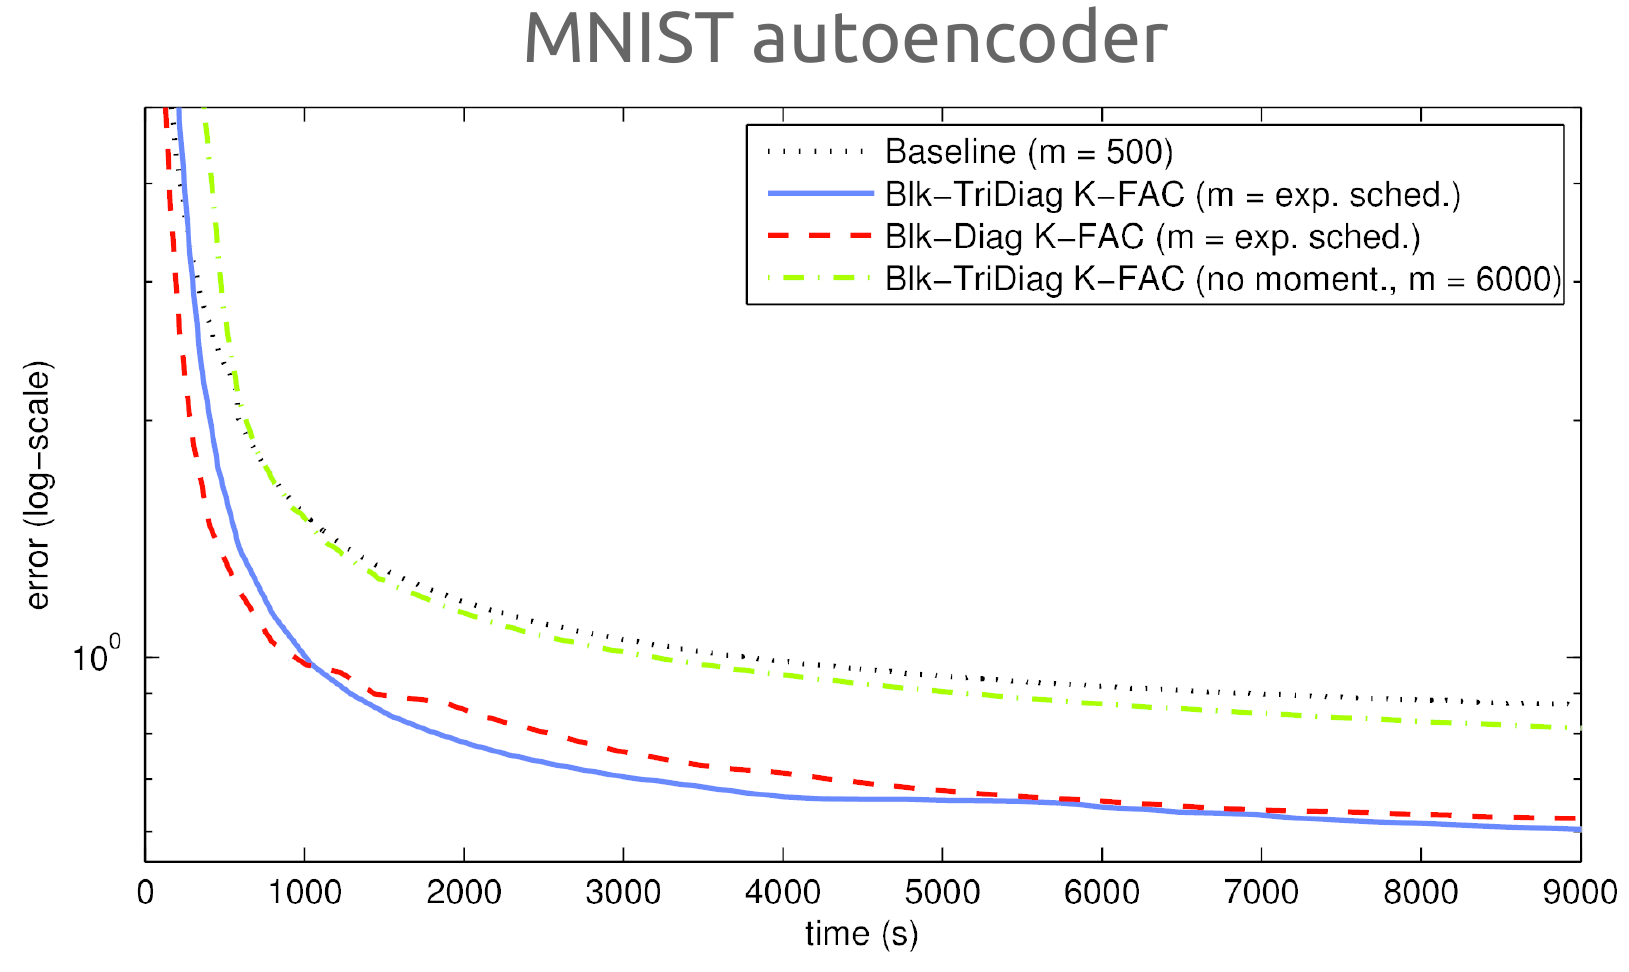
\includegraphics[scale=0.25]{mnist_autoencoder}
\end{figure}

\end{frame}
